% !TeX root = ../mat_mod2.tex

\section{
  Итерационный режим
  со случайным расположением вставок
  фиксированной~<<длины>>
}
\label{sect:5.5}
\setcounter{equation}{0}

Один из возможных подходов к решению проблемы выбора расположения оптимизирующей
вставки связан с организацией случайных испытаний.
Точнее, имеется в виду случайный выбор начала вставки.
На этой основе был построен вариант итерационного алгоритма,
краткое изложение которого приведено в настоящем разделе.

Итак, фиксируем
$\mathbf{k}\in \overline{0,\mathbf{n}-N}$
и допускаем возможность
случайного выбора начала вставки из <<интервала>> $\overline{0,\mathbf{k}}$.
Такой выбор осуществляется многократно,
что приводит к реализации итерационной процедуры.
Количество итераций может задаваться заранее или определяться
по мере достижения заданного качества.

Рассмотрим несколько этапов процедуры,
полагая, что на каждом из них выбор начала вставки осуществляется
на основе испытаний при использовании равномерного распределения.
Значение $N$ фиксировано.
Итак, пусть число
$\nu_1\in \overline{0,\mathbf{k}}$
получено как результат случайного испытания.
Далее используем процедуру, изложенную в \ref{sect:4.4} -- \ref{sect:4.7}
при условиях (\ref{5.4.4}),
где $(\lambda_0,h_0)$
соответствует (\ref{5.4.3})
и является ДР, определенным с помощью какого-либо эвристического алгоритма.
Использя
(\ref{4.4.13}), (\ref{4.4.14}) и (\ref{4.4.24})
в условиях (\ref{5.4.4}),
получаем ДР (\ref{5.4.5}) исходной <<большой>> задачи,
которое принимается за
$(\lambda_1,h_1)$
(см. (\ref{5.4.6})),
при этом реализуется неравенство (\ref{5.4.7}).

Теперь осуществляется случайное испытание,
результатом которого является
$\nu_2\in \overline{0,\mathbf{k}}$.
Вновь применяется процедура, изложенная
в \ref{sect:4.4} -- \ref{sect:4.7}
при условиях
$\lambda=\lambda_1$,
$(\mathbf{h}_i)_{i\in \overline{0,\mathbf{n}}}=h_1$ и
$\nu=\nu_2$
и доставляющая новое ДР
$(\lambda_2,h_2)$ <<большой>> задачи.
При этом реализуется неравенство
(\ref{5.4.10}).

Далее процедура повторяется,
доставляя в конце концов неравенство (\ref{5.4.11}),
где $\mathbf{r}\in \mathbb{N}$ определяет количество итераций.

В примере рассматривался случай
$\mathbf{n}=75$ и $|\mathbf{K}|=42$.
Размер вставок был выбран
$N=23$.
Функции стоимости предполагались такими же,
как в
\ref{sect:5.2}.
Количество итераций равнялось 15.
Начальный вариант был посчитан с использованием
эвристического итерационного алгоритма,
значение полученного критерия равно 259,51.
Результат, достигнутый после применения вставок на основе ДП, равен 257,16.
Общее время счета составляет 16 мин 11 с.
Маршрут и трасса показаны на рис.
\ref{DP_Random_Inserts_Result}.

\begin{figure}
  \begin{center}
  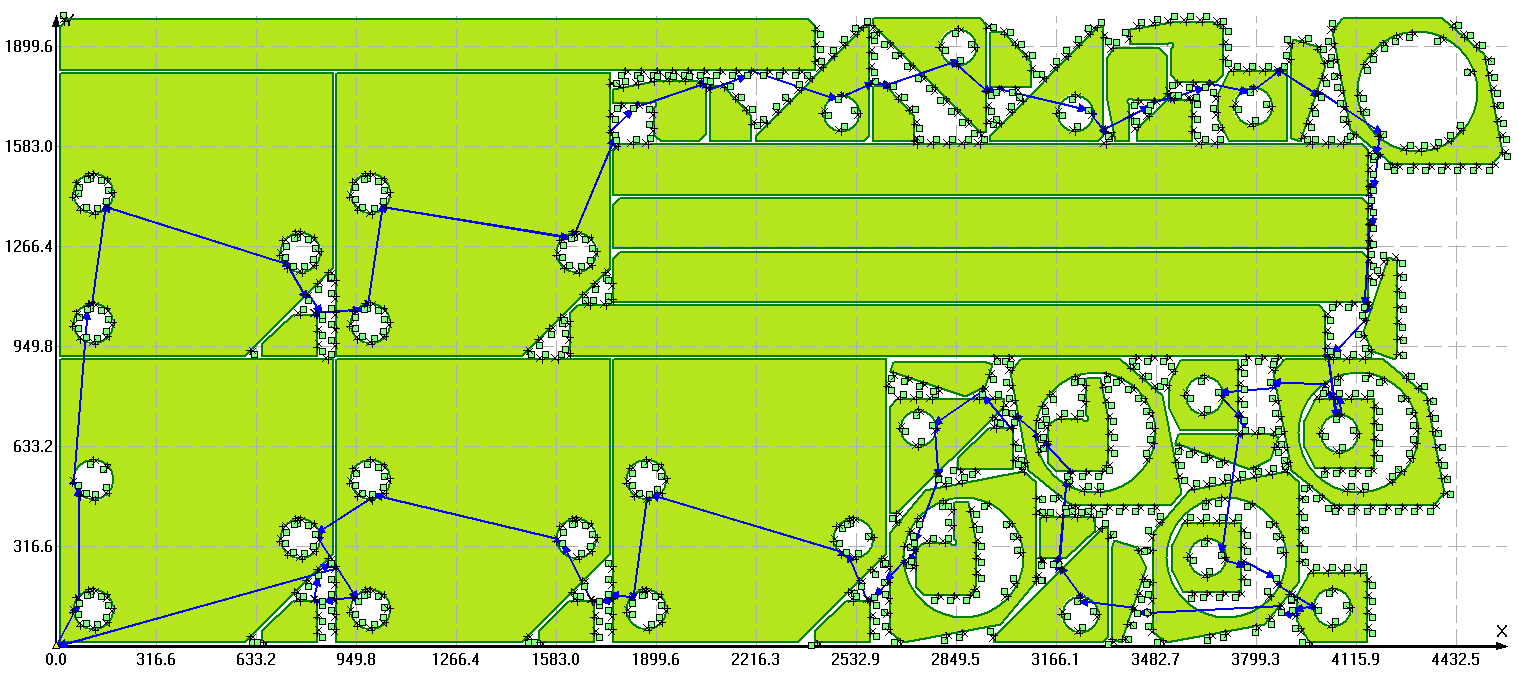
\includegraphics[width=0.9\textwidth]{route_random_dp_insertions.png}
  \caption{
    Траектория, полученная с использованием эвристического алгоритма
    с~улучшающими вставками на основе ДП (случайное расположение вставок)}
  \label{DP_Random_Inserts_Result}
  \end{center}
\end{figure}
